
\chapter{The key ideas}
% Maybe split into two chapters?

% Not too long, so that it can be read quickly

\section{Introduction -- what is this book about?}
Somebody who opens this book might wonder--is this book for me? What is this book about and will I benefit from reading it? Many readers might have heard about integrated nested Laplace approximation (INLA) and its that it is computationally efficiency and have picked up this book because it has INLA in the title in the hope of 
learning ``How to use INLA'' or what models can be fitted with the \texttt{R}-libraries \texttt{R-INLA} or \texttt{inlabru}. Others might have come across this book as they are familiar with INLA in a specific context and would now like to learn about a wider range of models that may be fitted with INLA. However, this book is not about INLA itself and about INLA as a model fitting method-- even though we provide some detail below--but as a means to an end. We are not going to discuss at length how INLA works as a method-- this has been discussed elsewhere. Discussing the methodology primarily through the maths behind it would mean looking at it from the point of view of a statistician, i.e.\ the method provider and hence someone who might want to understand mathematically what INLA does and why it is fast. 

In this book we take it for granted that INLA provides a computationally efficient and fast way of fitting a variety of practically relevant models and take on the point of view of the practitioners, the users of the methodology. For these, the analysis process does not start with a model fitting algorithm or a class of statistical models, but rather with the data collection process.  We discuss that the practitioner is interested in an underlying structure in nature, but when planning a study scientists need to initially think about how they can best gain information on and \textit{observe} this structure, bearing in mind the limitations and practicalities of data collection. As a result, statistical methodology has often often viewed through a specific data collection approach and accordingly, separate frameworks have been developed for each case. Here, the approach is to link different data collection methods to the underlying ``real'' structures and show that these are often very similar or even the same. This allows us to ``think'' in terms of the underlying structures, which in turn enables us to develop an approach that may be used to fit many different models within a single framework. This book is about that underlying structure--the spatial and temporal distribution of objects (such as individuals) or events (such as earthquakes)--and accounting for the different ways in which they have been observed.

When developing statistical methodology for many data structures, the spatial component that has traditionally not been explicitly pointed out or even discussed. 
This is different here --  we use spatial structure as a core concept -- it gets centre stage -- and show that the underlying structure in many data sets is the same. We can hence provide methods that allow us to fit a wide range of models conveniently within the same concept.

In this first chapter we show examples of a number of data structures for which methods relevant and hence can bee seen a typical special cases that the analysis methods discussed in this book can deal with. When reading this you may find that some of the data sets initially seem to be very different in structure. In this chapter we show the diversity and pointing out similarity.

Taking account of space and time- either as a nuisance or because it is of specific interest.

Notice that all examples below are plotted in space.

\section{Examples -- data structures}

Lets have a look at a few examples of common data structures. Together with some of the questions one might want to ask.

\subsection{Spatial point patterns}\label{subs:spp}
Figure \ref{fig:rainpattern} shows  a rainforest study plot 
%as Figure \ref{fig:elev}, 
detailing the spatial locations of trees of the species \textit{Beilschmidia} have been plotted. A study might be interested in analysing the pattern formed by those trees to understand habitat preferences of the species.  This data structure is referred to as a \textit{spatial point pattern}\index{spatial point pattern}.
\begin{figure}
\centering
%\includegraphics[width=0.3\textwidth]{complete}
%\includegraphics[width=0.6\textwidth]{sealsscotland}
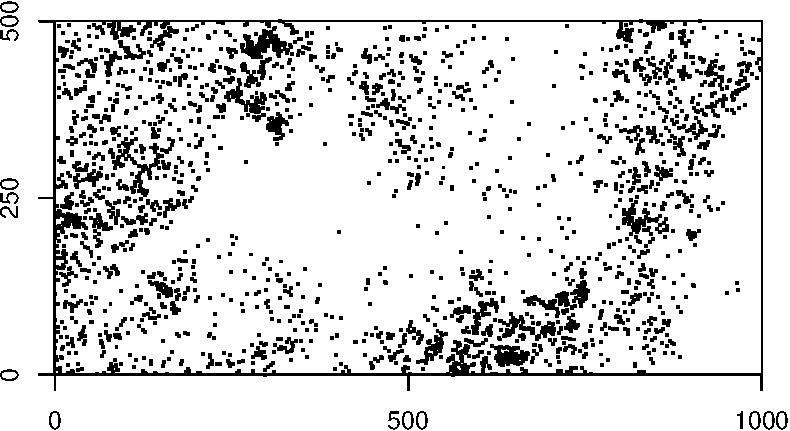
\includegraphics[width=0.6\textwidth]{rain_pattern}
\caption{\label{fig:rainpattern} Rainforest trees...}
\end{figure}

Similarly, Figure \ref{fig:earthquakes} shows the locations of earthquakes on the globe\footnote{Plot currently taken from %\texttt{http://eqseis.geosc.psu.edu/~cammon/HTML/Classes/IntroQuakes/
%Notes/plate_tect01.html}
}. 
\begin{figure}
\centering
%\includegraphics[width=0.3\textwidth]{complete}
%\includegraphics[width=0.6\textwidth]{sealsscotland}
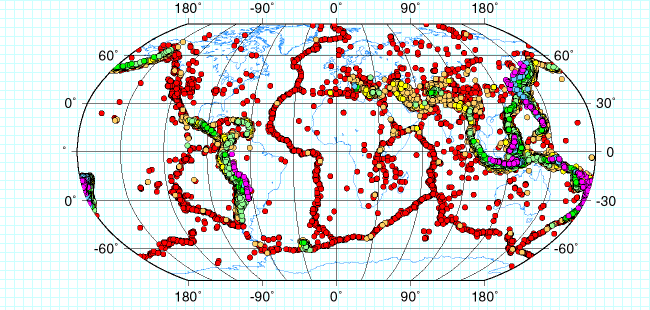
\includegraphics[width=0.6\textwidth]{earthquakes}
\caption{\label{fig:earthquakes} Pattern of earthquakes...}
\end{figure}
%Hence, unlike in the data structure in Section \ref{subsub:noindi} the locations have not been deliberately chosen as part of the study but are the object of interest. 
In an analysis, the main interest is to understand--and hence to analyse and model--the spatial pattern. For the rainforest  trees, spatial covariates on local topography and soil chemistry variables, might be used to associate tree aggregation with certain environmental conditions and hence explain the the spatial pattern. Earthquakes are well known to occur close to tectonic faults, and it is very clear from the the Figure that many of the earthquakes occur on lines that are likely to be faults. However, in both cases other mechanisms that are often less well understood contribute to the spatial pattern formed by the trees or the earthquakes--this \textit{additional spatial structure} in the pattern, which the covariates cannot explain. For appropriate statistical inference this remaining structure needs to be accounted for.

\subsection{Marked point patterns}
In many contexts there is an interest in analysing the occurrence of events in space and time as well as the events' properties. The pattern in Figure \ref{fig:bokoharam}, for instance, shows the locations of terrorist attacks in Xcountry between 1990 and 2005--where the size of the circle reflects the number of people killed for each of the events. In other words, we do not only know where an event took place but also have information on the death toll. This additional information--formally referred to as \textit{marks}--may be included in an analysis of a \textit{marked point pattern}\index{marked point pattern}. Interest in and whether it is related 

\begin{figure}
\begin{center}
\centerline{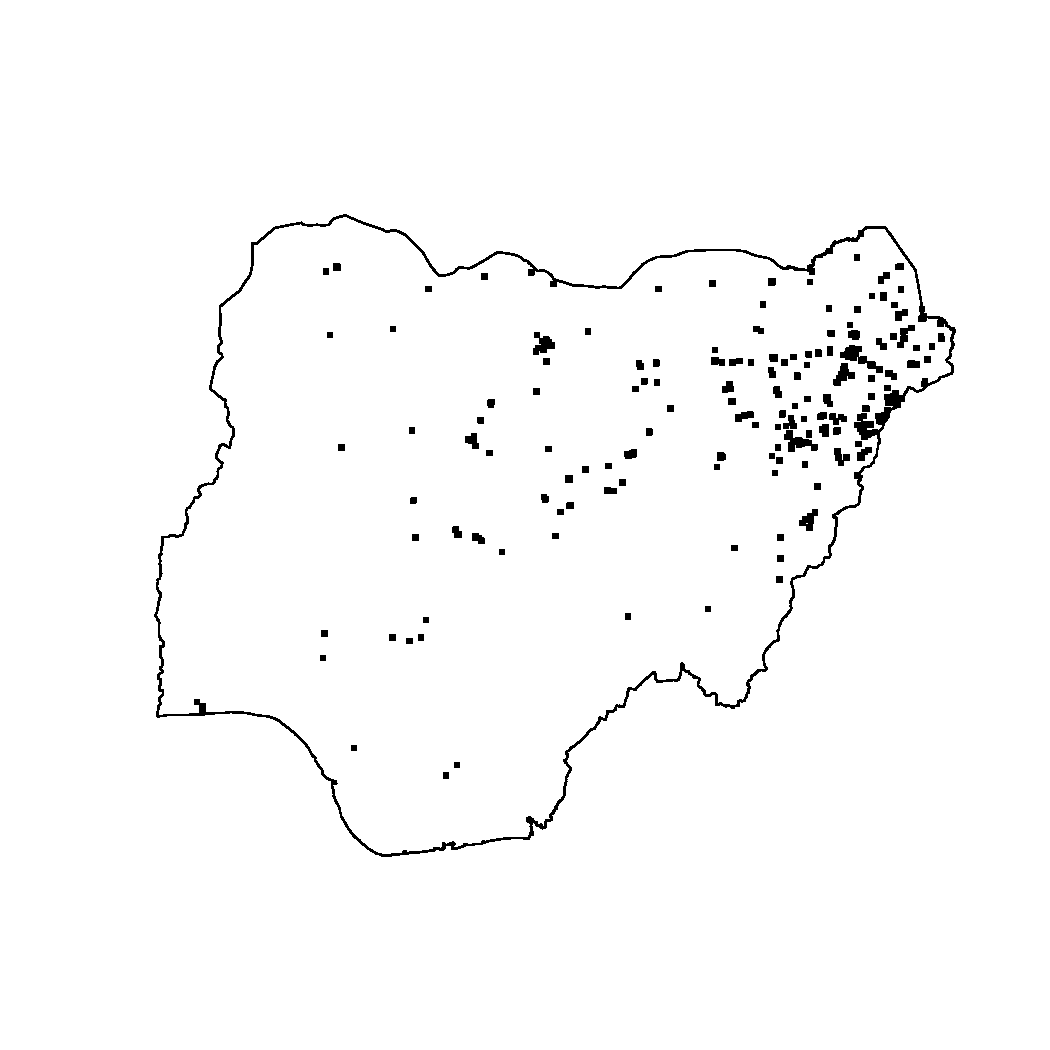
\includegraphics[width=10cm]{nigeria.pdf}}
\end{center}
\caption{Spatial pattern formed by the locations of terrorist attacks by the terror group Boko Haram in Nigeria from 2009 to 2014.}
\label{fig:bokoharam}
\end{figure}

We will discuss marked point pattern in detail

\subsection{Transect data}
In the case of the two datasets described in Section \ref{subs:spp}, information is available on the location of the trees and earthquakes for the entire area of interest. Researchers have been able to visit every single tree in the rainforest study plot  (above 10cm dbh), since it is feasible--if cumbersome--as the study area is ``only'' 50 hectare  in size. For the earthquake data modern  seismography allows geo-scientists to record earthquakes remotely. However, in other contexts is turns out to be more difficult to collect data and survey the whole area of interest.

Consider, for example, Figure \ref{fig:video} shows the location of transects used in a video survey of harbour porpoises off the East Coast of Scotland. 


\begin{figure}
\begin{center}
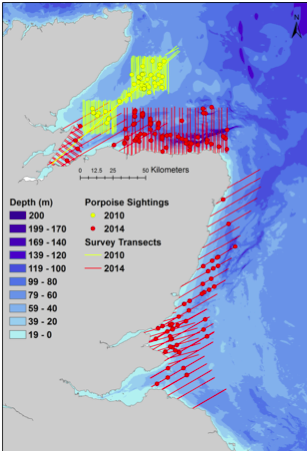
\includegraphics[width=0.3\textwidth]{videosurvey}
\caption{\label{fig:video} Pattern of transects...}
\end{center}
\end{figure}

Questions to ask - where and how many? To answer these questions one would like to survey the whole area, but this is not possible. 
In this book we will treat data of this structure as if it was a point pattern. To do this appropriately, we of course have to but take account of the  fact that we have not looked everywhere-- otherwise strongly underestimate the number of animals and get a very wrong idea of the spatial distribution. To do this, we adapt methodology that has been developed for patterns as the one in Figure \ref{fig:rainforest} and make the observation process explicit. This allows us to stay spatially explicit.

\subsection{Distance sampling data}
%Strip and point transects
In some context it is even more complicated...
Figure \ref{fig:dolphins} shows the locations of transects in the ocean laid out to spot cetaceans from a boat in a large study in the Eastern Tropical Pacific. 

Detection 
\begin{figure}
\begin{center}
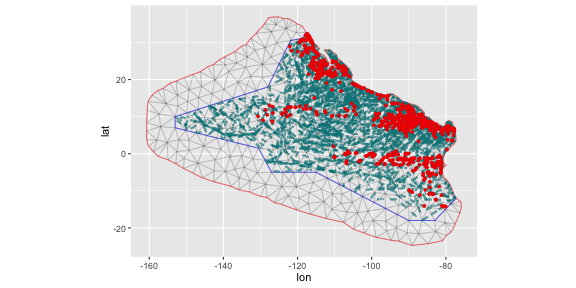
\includegraphics[width=0.70\textwidth]{dolphin}
\caption{\label{fig:dolphins} Pattern of dolphins...}
\end{center}
\end{figure}

Questions to ask - where and how many?


\subsection{Geo-referenced data}

\subsubsection{Spatially continuous data-- can't see individuals}\label{subsub:noindi}
\begin{figure}
\centering
%\includegraphics[width=0.3\textwidth]{complete}
%\includegraphics[width=0.6\textwidth]{sealsscotland}
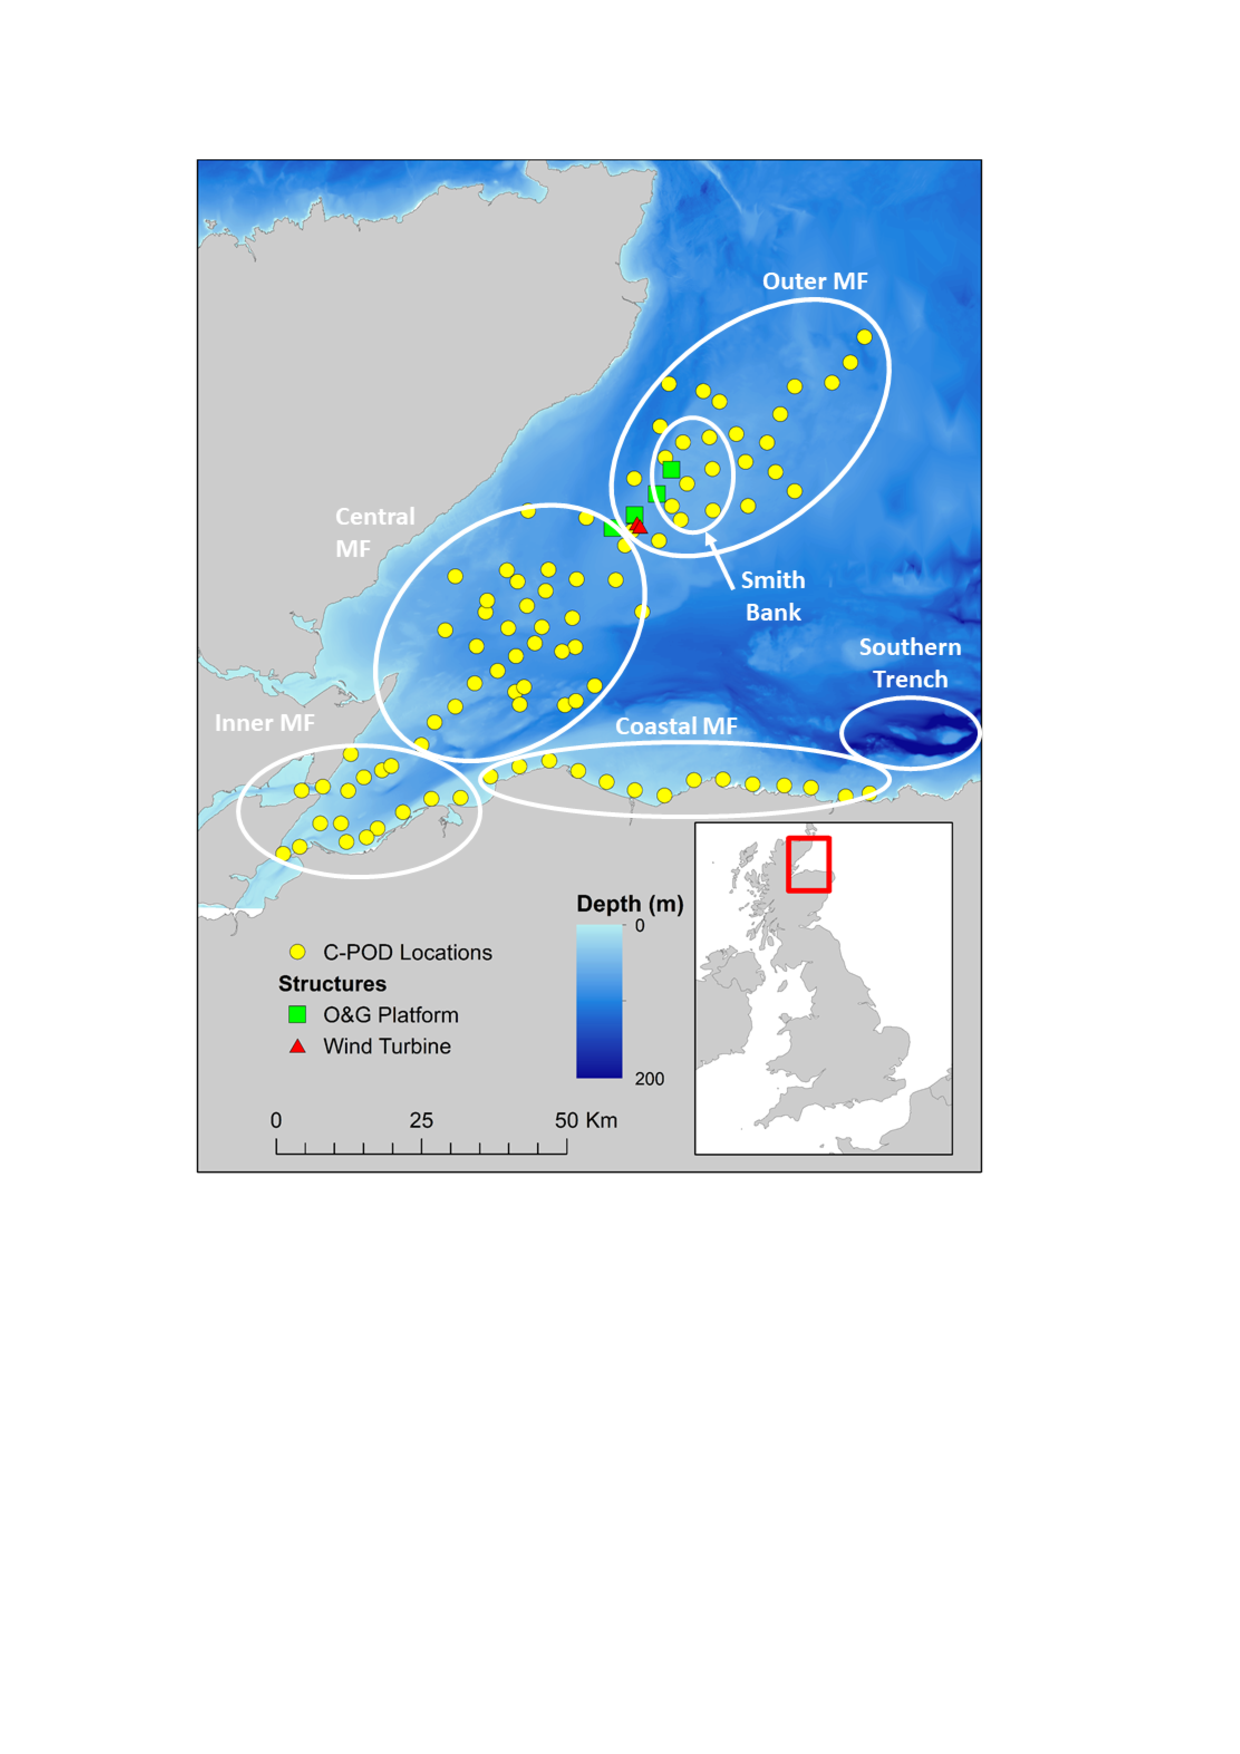
\includegraphics[width=0.4\textwidth]{cpodlocations}
\caption{\label{fig:elev} Some elevation somewhere...}
\end{figure}

\subsubsection{Spatially continuous data -- trap data}
Data collection -- trapping. Snap traps as in
Figure \ref{fig:voles} shows the location of traps. \footnote{plot from: Korpela K, Helle P, Henttonen H, Korpimäki E, Koskela E, Ovaskainen O, Pietiäinen H, Sundell J, Valkama J, Huitu O (2014) Predator–vole interactions in northern Europe: the role of small mustelids revised. Proceedings of the Royal Society B 281(1797): 20142119. https://doi.org/10.1098/rspb.2014.2119}

\begin{figure}
\centering
%\includegraphics[width=0.3\textwidth]{complete}
%\includegraphics[width=0.6\textwidth]{sealsscotland}
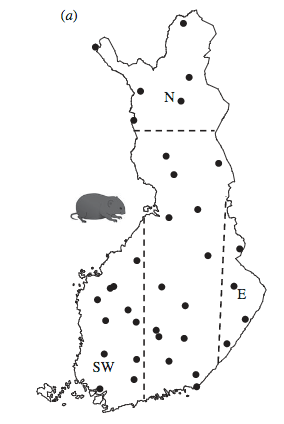
\includegraphics[width=0.4\textwidth]{voles}
\caption{\label{fig:voles} Locations of vole traps. Currently figure is a place holder -- taken from Korpela et al. 2014.}
\end{figure}




\subsubsection{Spatially continuous data---as covariates}

Consider Figure \ref{fig:elev}, which shows the elevation in a rainforest study plot in Panama. In this data structure that  takes on values everywhere in the plot; there is not a single location where it would not make sense to consider elevation as the quantity is spatially continuous.
\begin{figure}
\centering
%\includegraphics[width=0.3\textwidth]{complete}
%\includegraphics[width=0.6\textwidth]{sealsscotland}
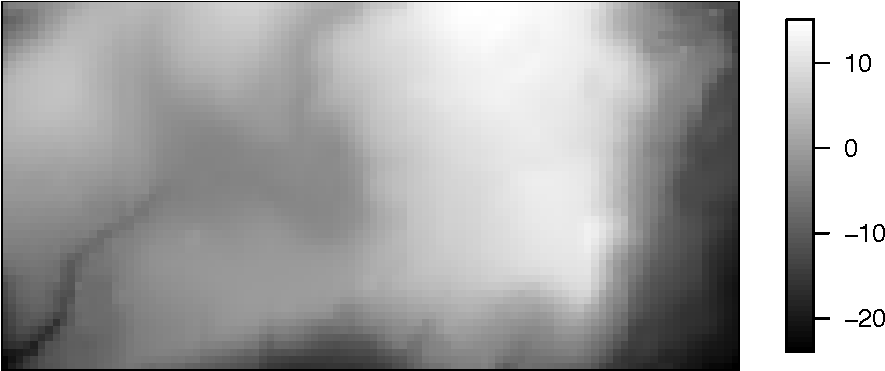
\includegraphics[width=0.6\textwidth]{elev}
\caption{\label{fig:elev} Some elevation somewhere...}
\end{figure}
In practice, however, there are limitations. While there are there are infinitely many locations in even a small area of space the quantity of interest cannot be measured everywhere in space -- and the quantity of interest cannot be fully observed. It can only be measured at a finite number of locations and these location have typically been chosen as part of the study design. There is an interest in interpolating to locations where no measurements have been taken -- referred to as \textit{spatial prediction}. This prediction into other areas of space needs to be done in a clever way, that take into account information from given measurements. In particular, on would like the predicted values to be similar to the values measured in the other locations. The figure is actually based on XX measurements in as many locations randomly distributed across the plot. There might also be an interest in relate one spatially continuous variable to other spatially continuous variables as part of a modelling exercise. These spatial covariates might help to explaining why values are high/low in different areas of the plot, but there might still be spatial structure left that needs to be accounted for.

This data structure is often referred to as \textit{geo-referenced data}\index{geo-referenced data} or \textit{geostatistical data}\index{geostatistical data}.


\subsection{Occupancy data}

%find good example

\section{Spatial data analysis}

\subsection{Spatial statistics -- dealing with spatial dependence}
Many ecological data sets are collected in the field rather than as part of a controlled experiment.  This has fundamental implications for the statistical analysis of these data sets since many factors and dependence structures that impact on the samples cannot be explicitly controlled for during data collection. Hence these have to be accounted for in the statistical analysis, which often implies that complex methodology has to be used.

More specifically, while standard statistical methodology assumes that samples are independent, samples collected as part of a field study are often spatially dependent. Ignoring the spatial dependence seriously impacts on the validity of any statistical inference drawn on the basis of  these data. This is because in standard statistical approaches, inference is made and conclusions are drawn based on assumptions on the distributional properties of the response variable of interest. These distributional properties however only hold for independent samples, given suitable covariates. Clearly, the assumption of independence no longer holds in spatially (or temporally etc.) dependent data. As a result, the entire inference process is flawed unless the statistical methodology explicitly accounts for the spatial dependence.  This is where \textbf{spatial statistics} comes in -- an area of statistics that seeks solutions to dealing with data that are inherently spatial and hence spatially dependent (or ``autocorrelated'').  Large parts of the spatial statistical literature aim at \textbf{accounting for spatial autocorrelation} in data to allow inference to be drawn from spatially dependent data.

However, spatial structure in a data set is not always a mere nuisance that needs to be accounted for before the variables of interest can be analysed. The main interest of a study may be in explicitly \textbf{analysing and modelling spatial structures}. Since spatial behaviour and spatial patterns may reflect important processes within an ecological community, some spatial statistical methods focus on the description of the information held in spatial dependence structures thus taking on an entirely different perspective.

In summary, spatial statistical methodology deals both with accounting for spatial dependence and with revealing spatial properties of a data set.  The models discussed in this book primarily focus on the latter as they are designed to provide an understanding of the spatial pattern formed by the locations of individuals in space -- the \textbf{spatial point pattern}. However, we will see that with increasing complexity of data sets and hence of models, both aims may be addressed within a single model allowing us to simultaneously use several levels of information contained in an ecological data set. This is done by both drawing on data observed in space while accounting for the spatial dependence and on information contained in the spatial structure itself.

\subsection{Spatial modelling -- computational challenges }

The \textbf{complexity} of many modern statistical models, and in particular that of models from within spatial statistics, implies that these are often difficult to fit and standard fitting methods used in classical statistics can only be used for the most basic (and often practically unrealistic) models. This is again due to the spatial dependence in the data  -- accounting for it tends to lead to likelihoods and distributions that are not analytically tractable and hence methods such as standard maximum likelihood approaches do not apply. As a result, fitting approaches are required that can handle complex likelihoods. 

Markov chain Monte Carlo (MCMC) has been used as a standard approach in recent decades. MCMC is a simulation based method which may be used to generate samples from complex distributions and may hence be used for inference when other methods fail. Unfortunately, our friend, the spatial dependence strikes again here. MCMC methods tend to be highly computationally demanding, in partic- ular for spatial models since accounting for spatial dependence in an MCMC simulation takes up a lot of computation time. This in turn quickly limits the level of complexity of the models that may realistically be fitted.
% particularly for data structures common in ecology.

Fortunately, however, Rue et al.\ 2009 recently developed  a different approach to dealing with  complex distributions that is based on \textbf{integrated nested Laplace approximation (INLA)}. INLA  avoids MCMC by approximating these distributions  and speeds up parameter estimation substantially.
This is great news for spatial statistics as it allows us to fit many spatial models within feasible time scales and hence to increase the complexity of models that can realistically be fitted. This is is \textit{also} great news for researchers who would like to  analyse their data while exploiting as much information contained in these to provide them with an improved understanding of their study system.  In general, INLA may be applied to a large class of statistical models -- \textbf{latent Gaussian models}. This class comprises many spatial as well as non-spatial models, see Rue et al.\ 2009. We discuss details of this model class in Chapter 2 -- for now it suffices to understand that many standard as well as complex and relevant models are in this class.. 



\section{Key concepts -- spatial point process and Gaussian random fields}

Datasets collected in different ways -- but the all have 
a spatial structure. Spatial structure is relevant, of interest or might impact on inference.
	
How do we represent this spatial structure? This is how 

\subsection{Spatial point processes -- models for point patterns}
Models that explain the patterns, why there are more points in some areas than in others. These models are stochastic models that are often referred to as \textit{spatial point processes} \index{spatial point process}

s, i.e.\ data sets that detail the exact spatial locations of individuals \footnote(these may be animals or plants -- or any other ``objects'',  including groups of individuals). Due to technological advances these are becoming increasingly available; these may be used to make inferences related to population and community structure and dynamics. The basic structure of these data sets consists of observations $\mathbf{x}=(x_1, \ldots, x_n)$ in two-dimensional (or higher dimensional) space. Spatial point process methodology seeks to describe and analyse spatial point patterns to infer information on the underlying mechanisms that generated these patterns. In this section we will briefly consider a few examples of data sets with increasing complexity and will return to these in detail in the individual analysis chapters.

A simple example of a spatial point pattern is the pattern plotted in Figure \ref{chap1:fig1}. It consists of the spatial locations of $251$ plants of the species \textit{Leucopogon striatus} collected as part of a study that assessed spatial pattern formation in a biodiverse plant community \citep{armstrong:91}.  This point pattern will be analysed with a relatively simple spatial model in Chapter 3 mainly to illustrate the basic modelling approach along with the relevant code in \texttt{R-INLA} and also to explicitly discuss the shortcomings of this simple model.
%\ref{chap3}
In this specific example, neither additional data on the plants forming the point pattern nor spatial covariates are available. As a result, the interpretation of the fitted model is limited and only provides information on the spatial trend in the point intensity. If spatial covariates as well as additional information on properties of each individual plant may be taken into account a model provides much more insight into underlying ecological processes and allows appropriate ecological interpretation. 

\begin{figure}[h]
\begin{center}
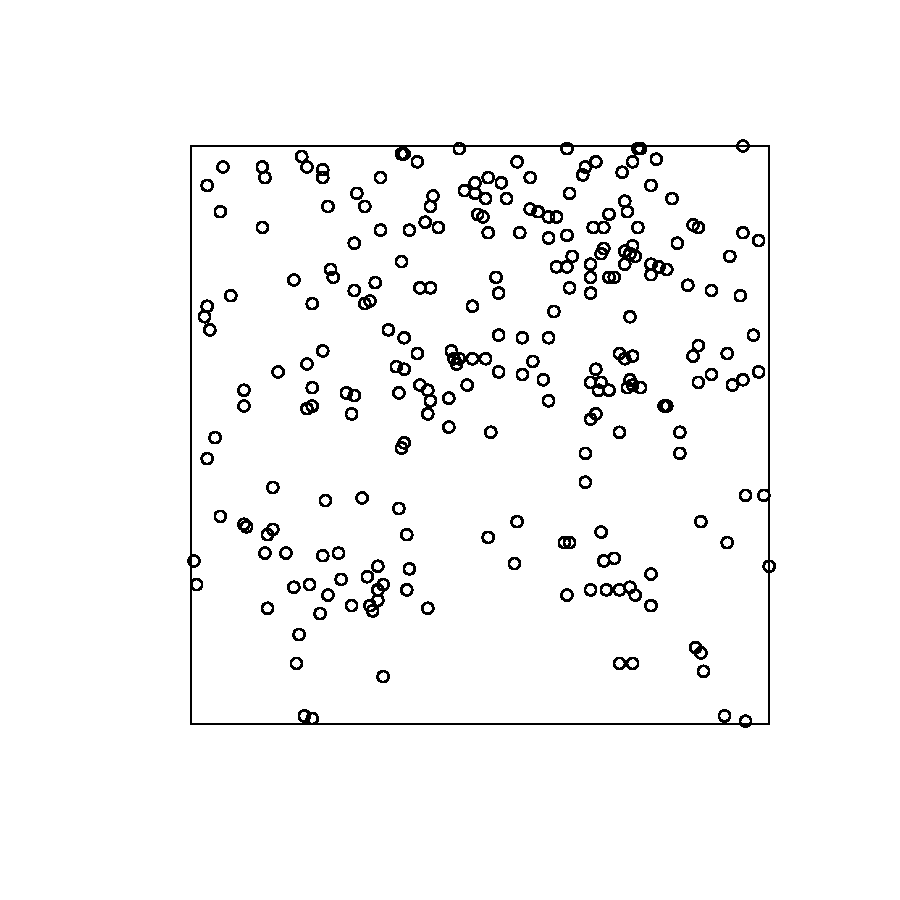
\includegraphics[width= 0.6\textwidth, angle= 0]{introduction-004}
\end{center}
\caption{The locations of $251$ plants of the species \textit{Leucopogon striatus} in a  $22\mbox{ m}$ $\times$ $22$ m area.}
\label{chap1:fig1}
\end{figure}

All other case studies hence deal with more complex examples which allow a more interesting and relevant model interpretation and are hence more relevant in the context of ecological data. This includes, for instance, an example for which several spatial covariates are available. These may be used to assess whether the spatial environment affects the presence or absence of individuals.  As an illustration, we analyse a data set in Chapter 4 that details the locations of rainforest trees of the species \textit{Protium Tenuifolium} in addition to a number of covariates that characterise the local habitat. Figure \ref{chap1:fig2} (a) shows a plot of this pattern.
%along with the soil variable ??? in Figure \ref{chap1:fig2} (b).
For this specific data set several soil variables are available and there is an interest in identifying which soil variables are most relevant for the presence of particular species. Methods for model comparison may be used to choose covariates, and we discuss the details and practicalities of this in Chapter 4.

\begin{figure}[h]
\begin{center}
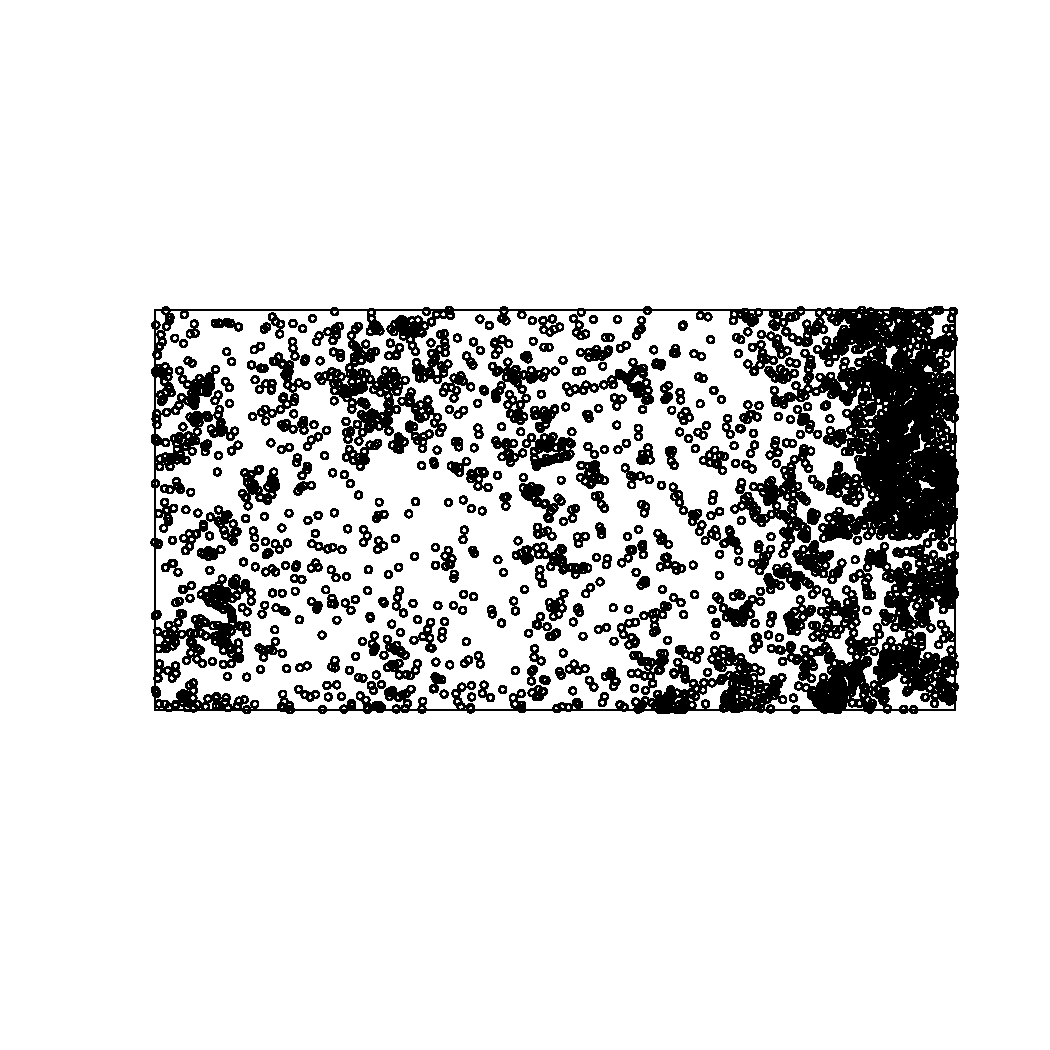
\includegraphics[width= 0.6\textwidth, angle= 0]{onetype}
\end{center}
\caption{The locations of $4294$ trees of the species \textit{Protium Tenuifolium} on a 50 ha plot on Barro Colorado Island, Panama.}
%and a plot of one soil variable!!!}
\label{chap1:fig2}
\end{figure}

However, by just treating each individual simply as a point -- and hence assuming that all individuals are the same -- may still appear too simplistic. In many ecological data sets, in addition to spatial location further information associated with each individual is available. These data may take on many different forms and may be qualitative (age class, species) or quantitative (size or age) and are referred to as \textbf{marks}.  Note that we conceptionally distinguish between (spatial) covariates and marks. Spatial covariates take on values in continuous space -- even if they cannot be measured everywhere in space. Marks are properties of the objects represented by the points. As such marks can only take on values in a location where an object is present -- it does not make sense to consider the height of a tree in a location where there is no tree. The discussions throughout the book will make it clear why this distinction is relevant and not only a formal one.

We will see through the case studies in Chapter 5-9 that very different types of questions may be addressed with different types of marked point pattern data. For instance, in the context of qualitative marks multi-type patterns may refer to individuals from different species. Here, one is often interested in understanding the co-occurrence of the different species  in space.  In Chapter 5 we discuss several approaches to a multi-type point pattern such as the the pattern in  Figure \ref{chap1:fig3} which shows the locations of the tree species \textit{Protium Tenuifolium} that we have already met in  Figure \ref{chap1:fig2} along with another species \textit{Tabernaemontana arborea}.
\begin{figure}[h]
\begin{center}
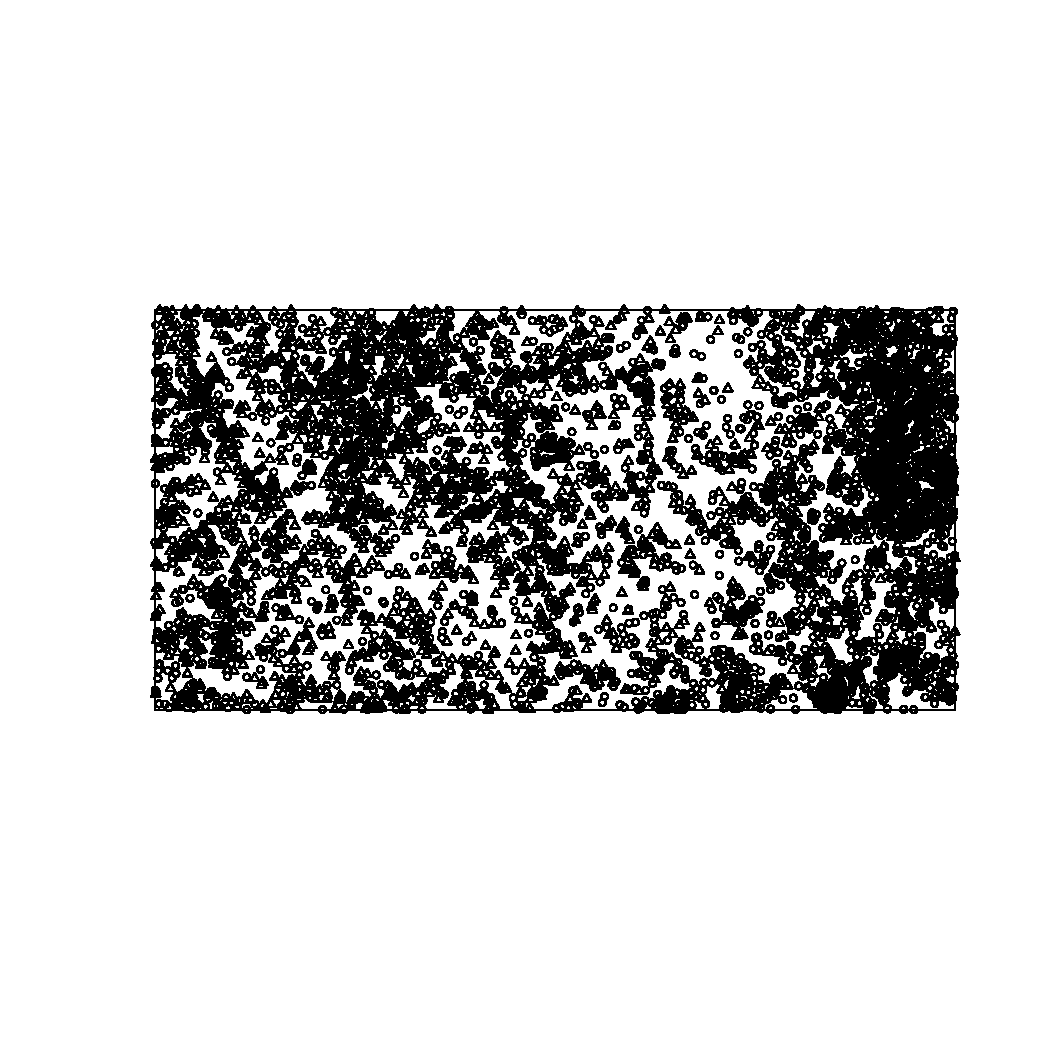
\includegraphics[width= 0.6\textwidth, angle= 0]{multitype}
\end{center}
\caption{The locations of 4294 trees of the species \textit{Protium Tenuifolium} (circles) and of 2213 trees of the species \textit{Tabernaemontana arborea} (triangles) in a 50 ha plot on Barro Colorado Island, Panama.}
%and a plot of the soil variable}
\label{chap1:fig3}
\end{figure}

In the context of quantitative marks one is often interested in assessing if the marks are related to the properties of the pattern itself. For example, trees may be smaller in areas where tree density is high but bigger where it is low. In addition, several marks may be available and these might depend on both the local intensity of the spatial pattern and on other marks. In Chapter 9 we discuss a model of eucalyptus trees (Figure \ref{chap1:fig4} (a)) for which chemical properties of the leaves (their palatability) are available  (Figure \ref{chap1:fig3} (b)), along with the frequency of use of the trees by koalas feeding on the leaves (Figure \ref{chap1:fig4} (c)). We assume that these two types of marks are dependent, and explicitly model the dependence along with the pattern itself, as well as the dependence of the pattern with the different marks. This type of model is computationally complex as it is a hierarchical model consisting of three (non-independent) levels with three separate likelihoods. Fitting a model of such a complexity with MCMC would be really time-consuming if not infeasible. We will show how such a model can be fitted with INLA in a straight forward way -- and will also show that the general structure of a hierarchical model with several dependent levels is a very versatile construction that may be used in many contexts, not only for marked point patterns.

 
\begin{figure}[!htb]
       \centering
    \begin{tabular}{c}
        \mbox{
            \subfigure[]{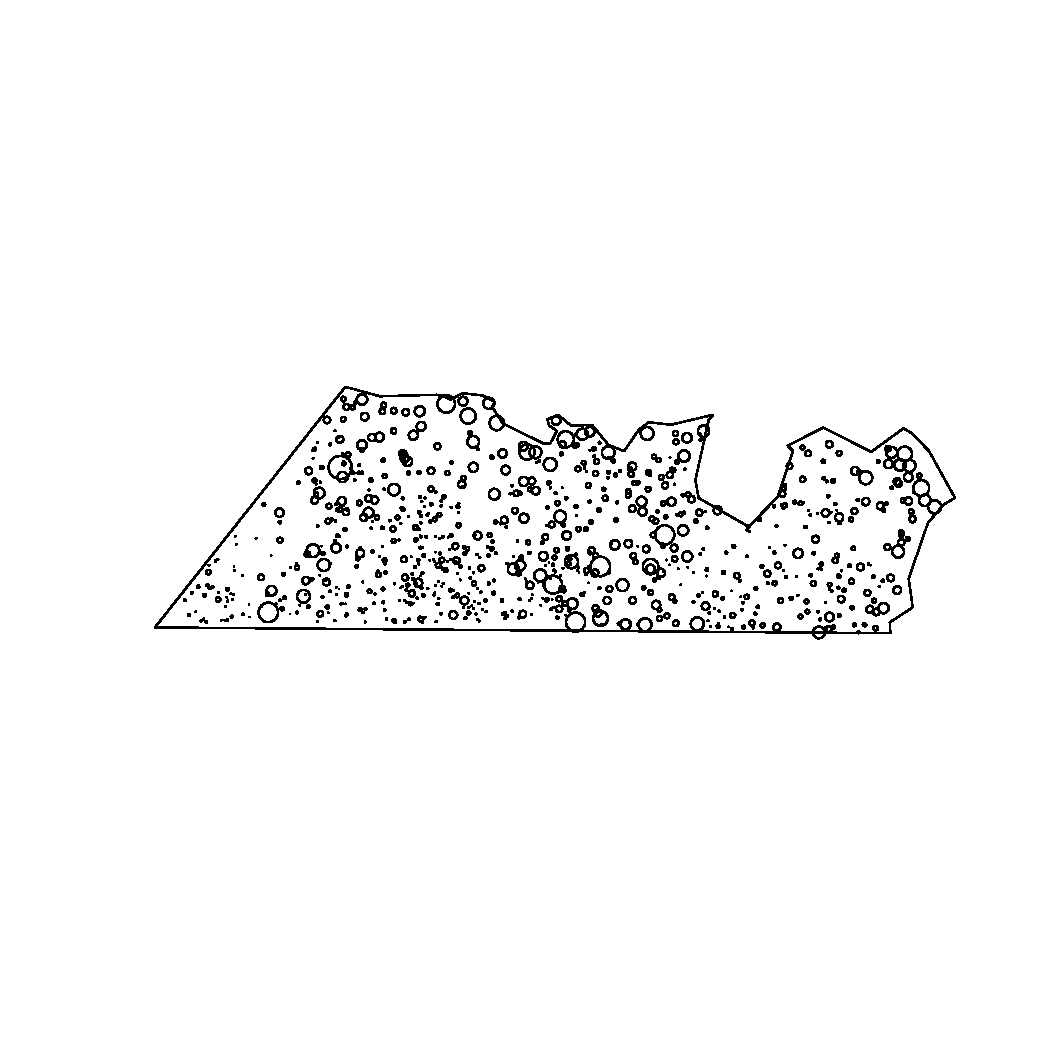
\includegraphics[width=10cm]{koala_food2_cut}}}\\
\mbox{
            \subfigure[]{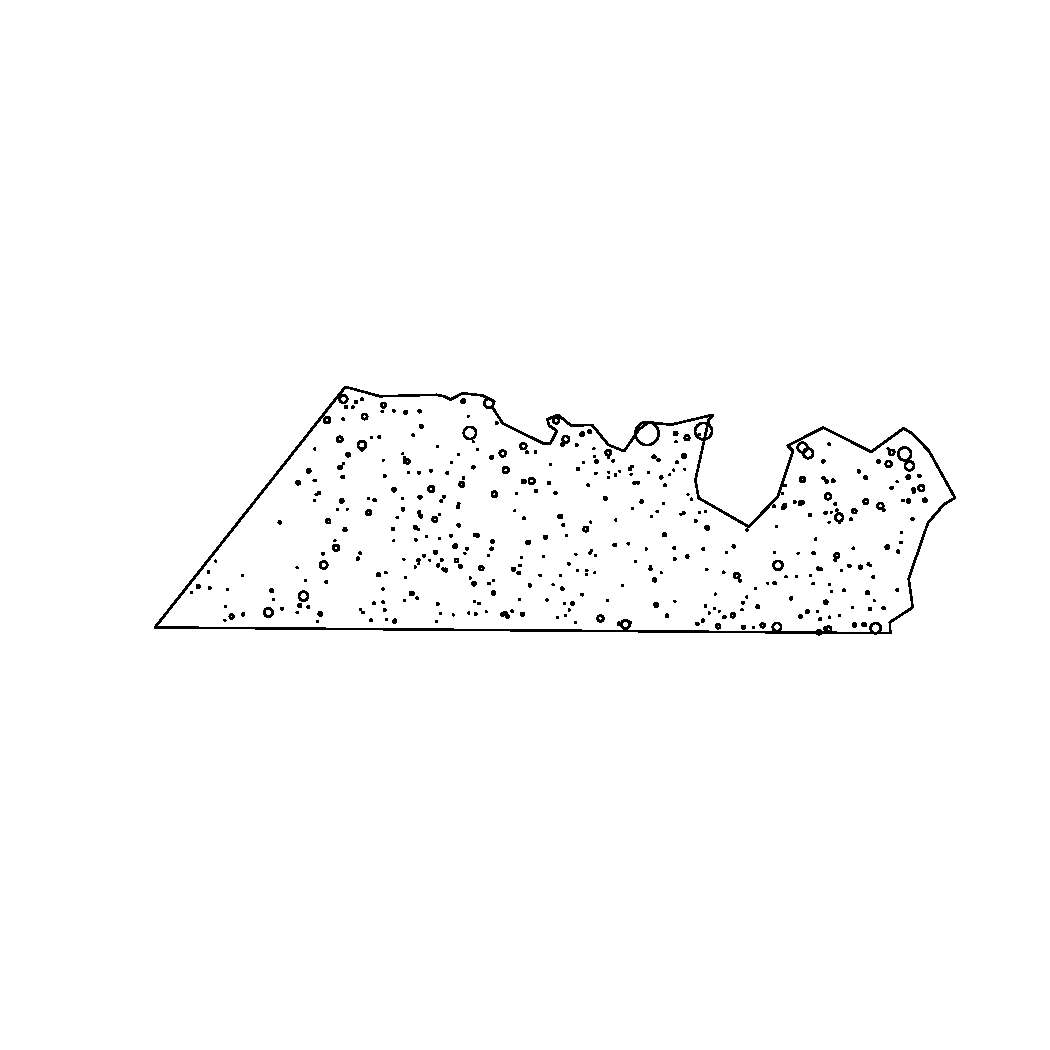
\includegraphics[width=10cm]{koala_freq2_cut}}}
    \end{tabular}
    \caption{Spatial pattern formed by the locations of the eucalyptus
        trees in the koala data set; the diameters of the circles
        reflect the value of the leaf marks (a) and the frequency
        marks (b) respectively.} 
\label{chap1:fig4}
\end{figure}

The patterns we have seen in this section should have given you an idea of some of the possible types of data sets that we will discuss -- and analyse ! -- in this book. However, before we embark on the concrete modelling of the different point patterns  provide some (only some!) background to the theory behind these models. This might on one hand help to understanding our objective better,  but also put the approaches discussed here into the context of existing literature.


\subsubsection{Mapped point processes versus thinned processes}

\subsection{Gaussian random fields--explaining remaining spatial structure}

remaining spatial structure




\section{Key tools -- GMRF and INLA}



\subsection{GMRF}

\subsection{INLA}
INLA (integrated nested Laplace approximation) is an alternative to MCMC
\begin{itemize}
\item much, much \textbf{faster}
\item  implemented in \texttt{R-INLA} 
%\item allows non-experts to fit complex models
\vspace{0.25cm}
\item suitable for a specific (but very large!) class of models
\end{itemize}

based on 
\begin{itemize}
\item Gaussian Markov random fields 
\item Latent Gaussian models
\item Laplace approximations 
\end{itemize}
$\Rightarrow$ very nice tool for Bayesian inference\\ 
$\Rightarrow$ computationally efficient model fitting, wide range of models
\begin{itemize}
\item quick 
\item accurate 
\item implemented in software \texttt{R-INLA}
%\item good scaling properties 
\end{itemize}

\subsection{SPDE}

Space is complex (sphere, holes) -- need to be flexible. Grids are rigid... 

Grid require binning, loss of information




\section{What to expect from the book}

Finding a rigorous yet flexible way of representing the spatial structure and linking this with computationally efficient model fitting strategies that allow us to fit relevant and realistically complex models.



\section{Structure of the book}

In the next Chapters we explore key concepts  -- spatial point patterns and random fields. It ends with a roadmap of this book.
 
Chapter after that formalises these concepts



